\Subsection{Билет 69: Комплексная диффернцируемость. Дифференцирование степенного ряда.}

\begin{definition} \thmslashn
	
	$f : E \mapsto \mathbb{C}$, $E \subset \mathbb{C}$, $z_0 \in \;$Int$ E$. Если существует $k \in \mathbb{C}$, такое что $f(z) = f(z_0) + k(z - z_0) + o(z - z_0)$ при $z \rightarrow z_0$, то $f$ -- \textcolor{red}{\textbf{комплексно-дифференцируема в точке}} $z_0$ и $k$ -- \textcolor{red}{\textbf{производная}} $f$ в точке $z_0$.
\end{definition}

\begin{remark} \thmslashn

	\begin{enumerate} 
		\item $k = \lim\limits_{z \to z_0} \frac{f(z) - f(z_0)}{z - z_0} =: f'(z_0)$
		\item Существование производной равносильно дифференцированию
	\end{enumerate}
\end{remark}

\begin{theorem} \thmslashn

	$R$ -- радиус сходимости ряда $f(z) = \sum\limits_{n = 0}^{\infty} a_n(z - z_0)^n$
	
	Тогда $f$ -- бесконечно дифференцируема в круге $|z - z_0| < R$ и
	
	$f^{(m)}(z) = \sum\limits_{n = m}^{\infty} n(n-1)\ldots(n-m+1)a_n(z-z_0)^{n-m}$
	\begin{proof} \thmslashn
	
		\begin{center}
			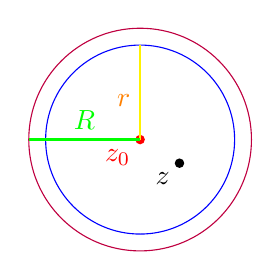
\begin{tikzpicture}[xscale=5, yscale=5]
			
				\filldraw[red] (0, 0) circle [radius=.3pt];
				\node[red, below left] at (0,0) {$z_0$};
			
				\draw[purple] (0,0) circle [radius=0.2828];
				\draw[blue] (0,0) circle [radius=0.24];
			
				\draw [yellow, thick, -] (0,0) -- (.0,.24);
				\node[orange, left] at (.0,.1) {$r$};
				
				\draw [green, thick, -] (0,0) -- (-0.2828,.0);
				\node[green, above] at (-0.1414,.0) {$R$};
			
				\filldraw[black] (.1,-0.06) circle [radius=.3pt];
				\node[below left] at (.1,-0.06) {$z$};
			
			\end{tikzpicture}
		\end{center}
		Докажем индукцию по $m$. Рассмотрим $m = 1$ и $z_0 = 0$ (про $z_0$ для простоты). Возьмем $|z| < R$ и подберем такое $r$, что $|z| < r < R$ (картинка выше для пояснения). Возьмем $|w| < r$
		\[
		f'(z) = \lim\limits_{w \to z} \frac{f(w) - f(z)}{w - z} = \lim\limits_{w \to z} \sum\limits_{n=0}^{\infty} \frac{a_nw^n - a_nz^n}{w-z} = \lim\limits_{w \to z} \sum\limits_{n=1}^{\infty} a_n (w^{n-1} + w^{n-2}z + \cdots + z^{n-1})
		\]
		Первое равенство -- просто вынесли ряд. Второе -- просто поделили (что-то похожее на алгебре делали). Осталось доказать равномерную сходимость по $|w| < r$ последнего ряда, чтобы поменять местами предел и сумму. Проверять будем с помощью признака Вейерштрасса:
		\[
		|a_n(w^{n-1}+w^{n-2}z+\cdots + z^{n-1})| \leqslant |a_n|(|w|^{n-1}+|w|^{n-2}|z|+\cdots + |z|^{n-1}) \leqslant |a_n|nr^{n-1}
		 \]
		 Второе неравенство, так как $|w| < r$ и $z < r$. Но ряд $\sum\limits_{n=1}^{\infty} |a_n|nr^{n-1}$ сходится, так как у ряда $\sum\limits_{n=1}^{\infty} a_nnz^{n-1}$ радиус сходимости $R > r$. Значит применился признак сходимости и мы можем поменять местами сумму с предлом.
		 \[
		 \lim\limits_{w \to z} \sum\limits_{n=1}^{\infty} a_n (w^{n-1} + w^{n-2}z + \cdots+ z^{n-1}) = \sum\limits_{n=1}^{\infty}  \lim\limits_{w \to z} a_n (w^{n-1} + w^{n-2}z + \cdots+ z^{n-1}) = \sum\limits_{n=1}^{\infty} na_nz^{n-1}
		 \]
		 Если применить эту форму $m$ раз, то получим искомую формулу.
	\end{proof}
\end{theorem}